\section{Execution}
\label{sec:execution}

A picture of the setup can be seen in \autoref{fig:setup}.

\begin{figure}[H]
    \centering
    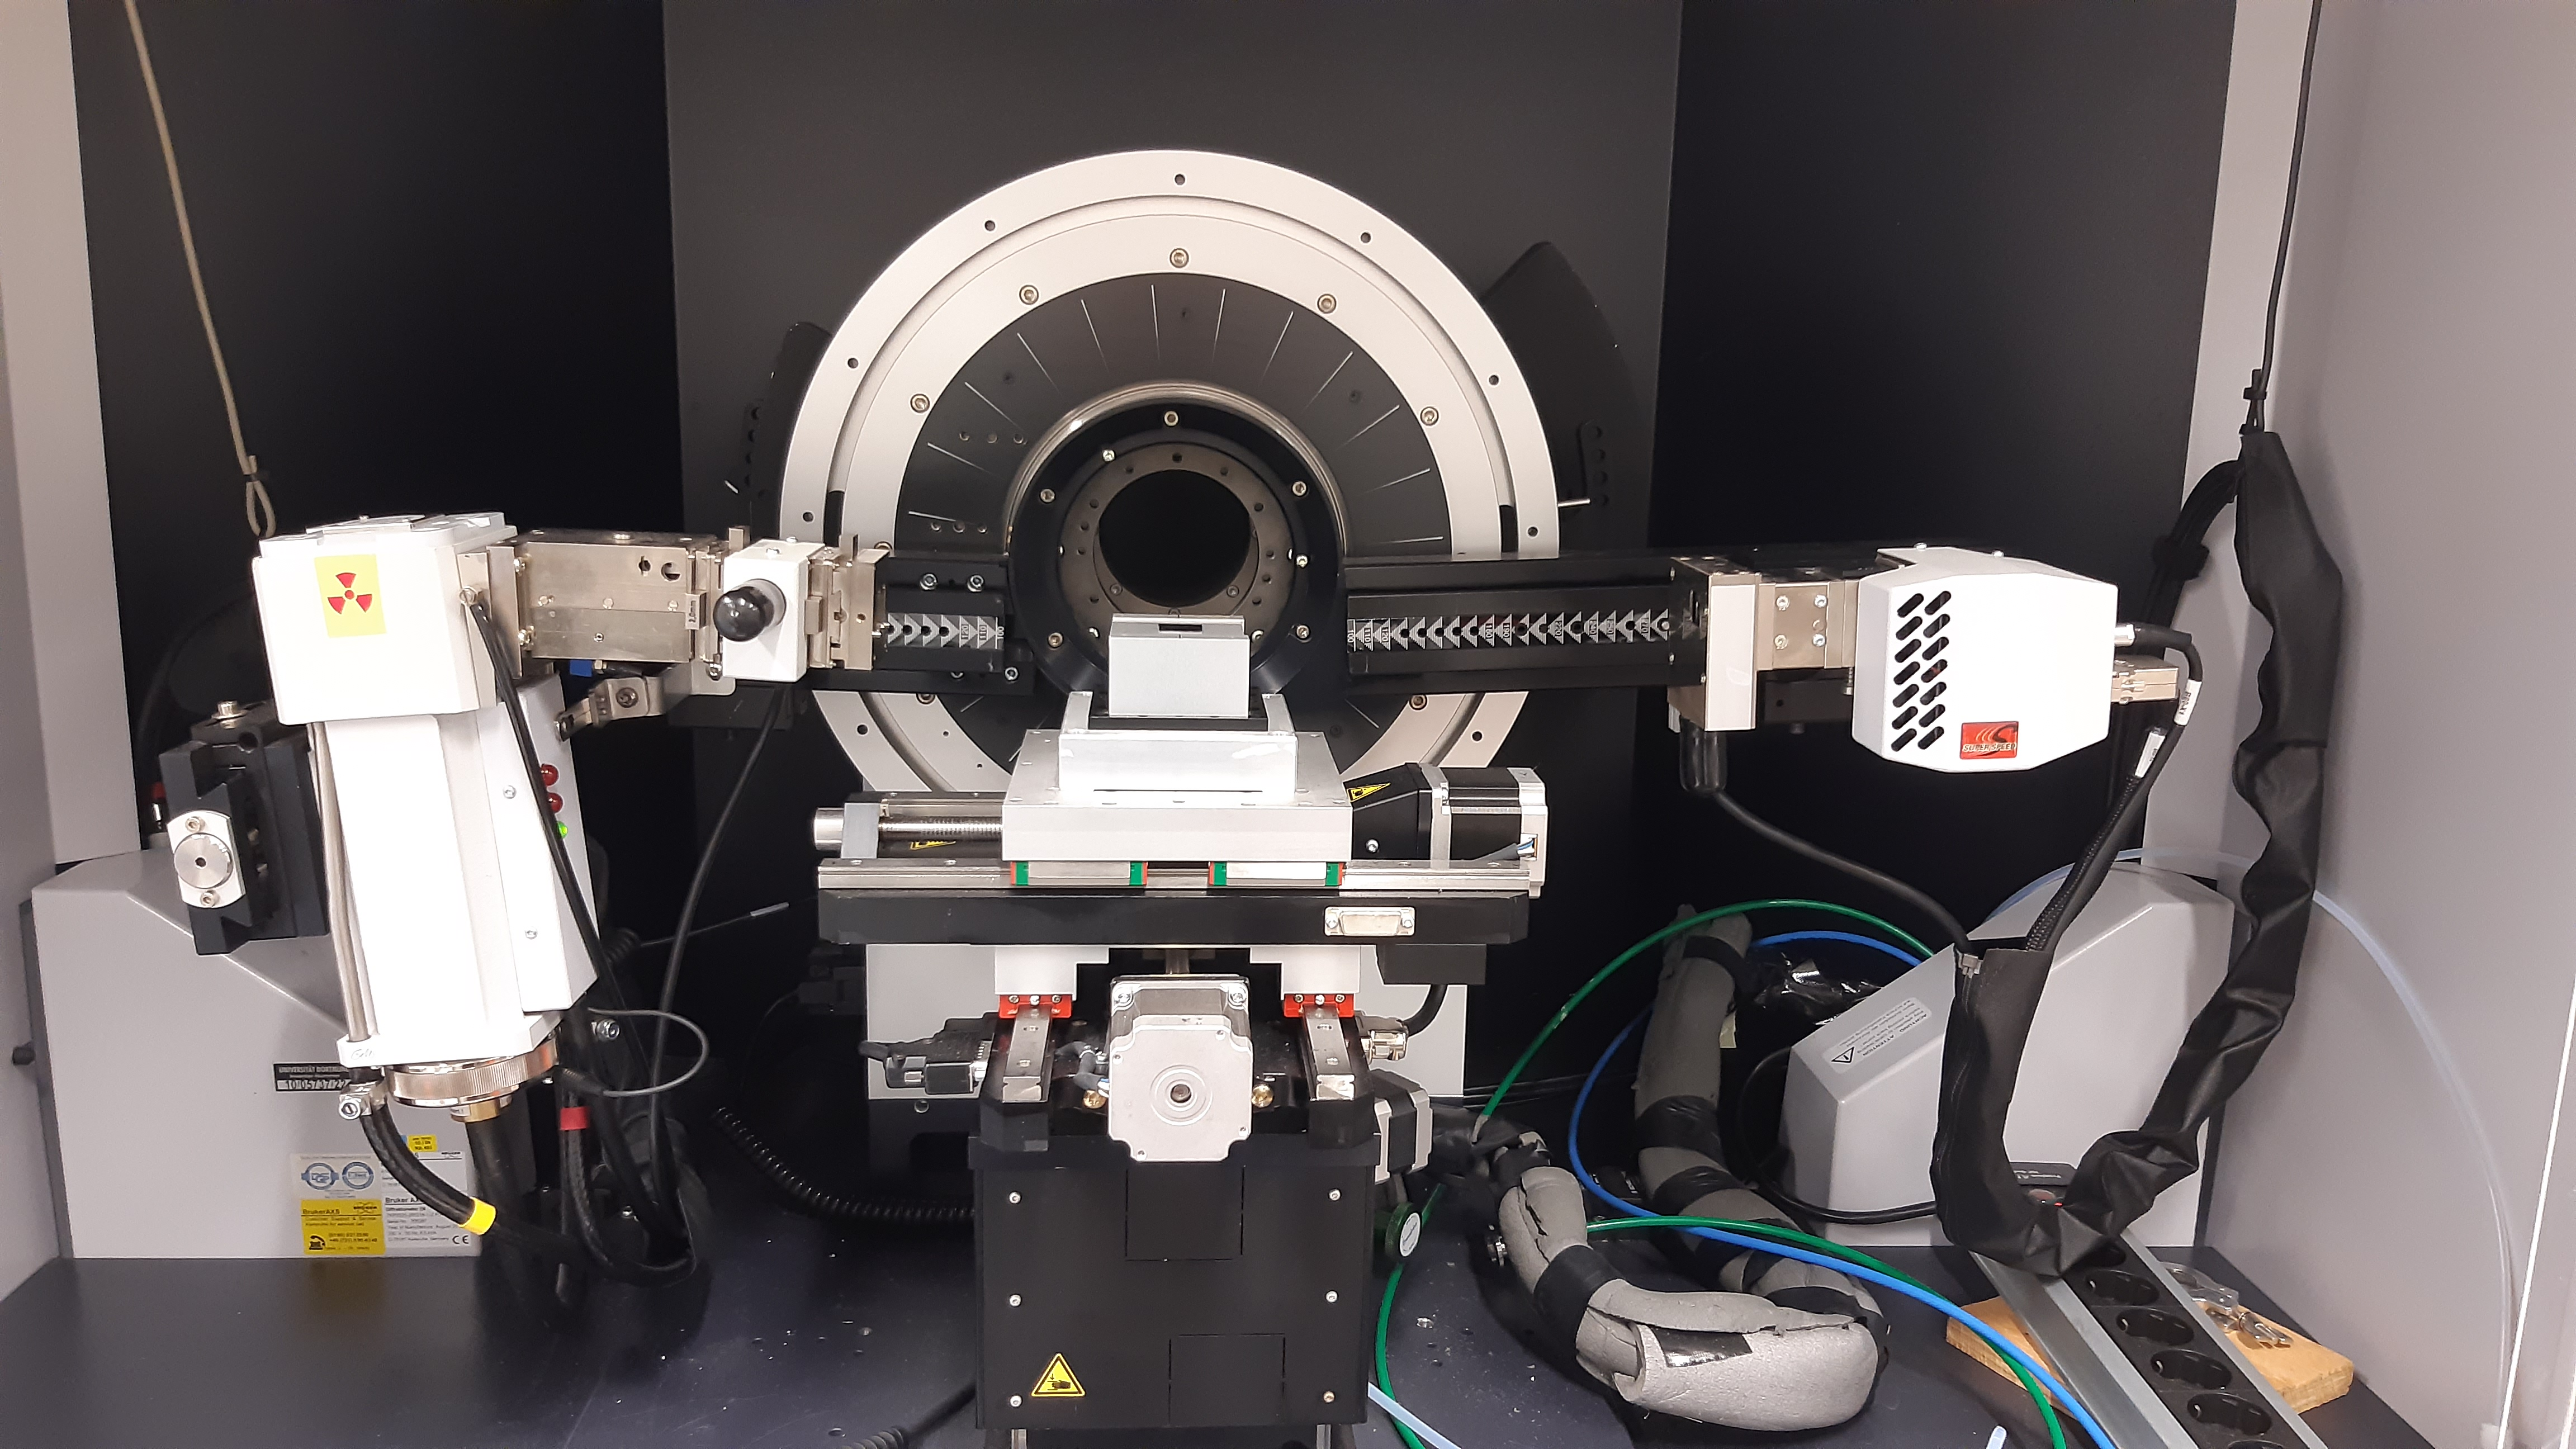
\includegraphics[width = .8\textwidth]{figures/aufbau.jpg}
    \caption{A photograph of the setup used in this experiment. On the left is the X-ray source and on the right the detector with the sample in the middle.}
    \label{fig:setup}
\end{figure}

To perform the experiment, a D8 laboratory diffractometer from Bruker-AXS is used.
The measurements themselves as well as drive control is being taken care of by the software XRD Command.
As explained, the X-rays are created in an X-ray tube and then hit the Göbel mirror, 
a mirror specifically created to parallelise X-rays, since the tube emits them evenly throughout every direction.
Then, the X-rays hit the sample and are reflected so that they can enter the detector. \\

This arrangement, however, has to be adjusted before the real measurement can be started.
In order to do that, a multitude of scans is performed as shown in \autoref{fig:scans}.

\begin{figure}[H]
    \centering
    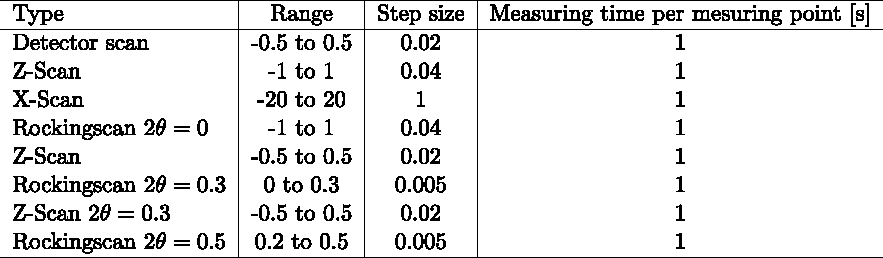
\includegraphics{figures/scans.pdf}
    \caption{A table showing the different scans that have to be performed in order to align the sample and the detector, 
    including the recommended settings for XRD Command \cite{v44}.}
    \label{fig:scans}
\end{figure}

As can be seen from the number of scans that need to be performed, it is important that the sample is aligned just right with the detector.
<<<<<<< HEAD
Before beginning the sample alignment, the primary beam is adjusted.
To do that, the sample is moved out of the beam by changing the z-coordinate and a detector scan is performed.
This moves the detector in a small angular range, yielding a scan in the form of a Gaussian.
the Gausssian's maximum is then chosen to be the new zero position of the detector. \\
Now, the sample alignment can begin.
The z-coordinate is aligned by moving the sample through the X-ray until it blocks half the intensity.
||||||| 1cda87c
First the z-coordinate is aligned by moving the sample through the X-ray until it blocks half the intensity.
=======
First, the z-coordinate is aligned by moving the sample through the X-ray until it blocks half the intensity.
>>>>>>> 6c03826f83bc9db80ef11dc8d64c059fe86281c8
When adjusting the x-coordinate a plateau should show in the X-Scan.
The middle of the plateau is chosen and the sample is moved there via the diffractometer's drives.
After that, aRockingscan is performed to adjust the y-coordinate, which, as well as the Z-Scan, is performed multiple times at
different angles to ensure high precision.
The Rockingscan gives information about the tilt of the sample relative to the X-ray beam.
A correctly performed Rockingscan should yield a symmetrical triangle.
This means that both the z-coordinate is aligned properly and that the sample is hit directly in its center of rotation of the diffractometer. \\

After the alignment, the measurements are performed.
First, an \textbf{Omega/2Theta}-type scan with a range of $0°$ to $\SI{2.5}{\degree}$ and a step size of $\SI{0.005}{\degree}$ with $\SI{5}{\second}$ per step is performed.
Then, to measure the diffuse background, the detector is tilted by $\SI{0.2}{\degree}$ and the same measurement is performed again.


